\documentclass[12pt,a4paper]{article}
\usepackage[utf8]{vietnam}
\usepackage{amsmath,amssymb}
\usepackage{tabularx}
\usepackage{tikz}
\usetikzlibrary{calc,angles,quotes,arrows.meta,patterns}
\usepackage{xcolor}
\usepackage{enumitem}
\usepackage{fancyhdr}
\usepackage{graphicx}
\usepackage[top=1.0cm, bottom=1.0cm, left=1.2cm, right=1.2cm]{geometry}
\usepackage[dethi]{ex_test}
\SAOPTN{widthSA=3.2,heightSA=0.62}

\setlength{\headheight}{15pt}
\setlength{\parskip}{0pt}

\pagestyle{fancy}
\fancyhf{}
\rhead{\textit{Môn Toán 8 -- Đề số 07}}
\lhead{\textit{Bộ đề ôn tập Giữa học kì I}}
\cfoot{\thepage}

\begin{document}

% --- KHUNG TIÊU ĐỀ ĐỀ THI ---
\noindent
\begin{tabularx}{\linewidth}{X r}
\textbf{TRƯỜNG THCS: \dotfill} & \textbf{ĐỀ KIỂM TRA ĐỊNH KỲ GIỮA HỌC KỲ I} \\
\textbf{Họ và tên: \dotfill} & \textbf{NĂM HỌC 2026 -- 2027} \\
\textbf{Lớp: \dotfill \quad SBD: \dotfill} & \textbf{Môn: TOÁN 8} \\
\hline
\end{tabularx}
\vspace{2mm}

\begin{center}
  \textbf{\large ĐỀ ÔN TẬP GIỮA HỌC KỲ I -- ĐỀ SỐ 07}\\
  \textit{Thời gian làm bài: 90 phút (Không kể thời gian phát đề)}
\end{center}
\vspace{1mm}

% --- PHẦN I ---
\noindent\textbf{\large PHẦN I. CÂU TRẮC NGHIỆM NHIỀU PHƯƠNG ÁN LỰA CHỌN (3,0 điểm)}

\textit{Thí sinh trả lời từ câu 1 đến câu 12. Mỗi câu hỏi thí sinh chỉ chọn một phương án duy nhất.}

\vspace{1mm}
\begin{ex}
Trong các biểu thức sau, biểu thức nào không phải là đơn thức?
\choice
{$-2xy^2$}
{$7$}
{\True $x + 2y$}
{$3xy$}
\end{ex}

\begin{ex}
Cặp đơn thức nào sau đây là hai đơn thức đồng dạng?
\choice
{$2x^2y$ và $2xy^2$}
{\True $-3x^3y^2$ và $5x^3y^2$}
{$4x^2$ và $4x^3$}
{$2xy$ và $xy^2$}
\end{ex}

\begin{ex}
Bậc của đa thức $Q = x^2y^4 - 3x^5y + 2x^2y - 5$ là:
\choice
{\True 6}
{5}
{4}
{3}
\end{ex}

\begin{ex}
Kết quả của phép nhân $-3x^2 \cdot (2x - y)$ là:
\choice
{$-6x^3 - 3x^2y$}
{\True $-6x^3 + 3x^2y$}
{$-6x^2 + 3x^2y$}
{$6x^3 - 3x^2y$}
\end{ex}

\begin{ex}
Biểu thức $x^2 - 4y^2$ được viết dưới dạng tích là:
\choice
{$(x - 2y)^2$}
{$(x - 4y)(x + 4y)$}
{\True $(x - 2y)(x + 2y)$}
{$(x + 2y)^2$}
\end{ex}

\begin{ex}
Đa thức $x^2 - 6x + 9$ được viết dưới dạng bình phương của một hiệu là:
\choice
{\True $(x - 3)^2$}
{$(x + 3)^2$}
{$(x - 9)^2$}
{$(x + 9)^2$}
\end{ex}

\begin{ex}
Kết quả của phép tính $(-15x^3y^4) : (3xy^2)$ là:
\choice
{\True $-5x^2y^2$}
{$5x^2y^2$}
{$-5x^4y^6$}
{$-5x^2y$}
\end{ex}

\begin{ex}
Cho tứ giác $EFGH$ có $\widehat{E} = 70^\circ$, $\widehat{F} = 110^\circ$, $\widehat{G} = 80^\circ$. Số đo góc $H$ là:
\choice
{\True $100^\circ$}
{$90^\circ$}
{$80^\circ$}
{$110^\circ$}
\end{ex}

\begin{ex}
Tứ giác có các cạnh đối song song là:
\choice
{Hình thang}
{\True Hình bình hành}
{Hình chữ nhật}
{Hình thoi}
\end{ex}

\begin{ex}
Hình bình hành có hai đường chéo vuông góc với nhau là:
\choice
{Hình chữ nhật}
{Hình thang cân}
{\True Hình thoi}
{Hình vuông}
\end{ex}

\begin{ex}
Mặt đáy của hình chóp tam giác đều là hình gì?
\choice
{Tam giác cân}
{Tam giác vuông}
{\True Tam giác đều}
{Tam giác vuông cân}
\end{ex}

\begin{ex}
Cho hình chóp tam giác đều có độ dài cạnh đáy bằng $4\text{ cm}$ và độ dài trung đoạn bằng $9\text{ cm}$. Diện tích xung quanh của hình chóp đó là:
\choice
{\True $54\text{ cm}^2$}
{$108\text{ cm}^2$}
{$36\text{ cm}^2$}
{$27\text{ cm}^2$}
\end{ex}


\vspace{1mm}
\noindent\textbf{BẢNG TRẢ LỜI TRẮC NGHIỆM PHẦN I:}
\begin{center}
\begin{tabular}{|c|c|c|c|c|c|c|c|c|c|c|c|c|}
\hline
\textbf{Câu} & \textbf{1} & \textbf{2} & \textbf{3} & \textbf{4} & \textbf{5} & \textbf{6} & \textbf{7} & \textbf{8} & \textbf{9} & \textbf{10} & \textbf{11} & \textbf{12} \\
\hline
\textbf{Chọn} & \rule{0pt}{0.65cm} & & & & & & & & & & & \\
\hline
\end{tabular}
\end{center}
\vspace{2mm}

\setcounter{ex}{0}
\noindent\textbf{\large PHẦN II. CÂU TRẮC NGHIỆM ĐÚNG SAI (2,0 điểm)}

\textit{Thí sinh trả lời câu 1 và câu 2. Trong mỗi ý a), b), c), d) ở mỗi câu, thí sinh chọn đúng hoặc sai.}

\vspace{1mm}
\begin{ex}
Cho biểu thức $A = \left(\dfrac{x}{x^2 - 4} + \dfrac{1}{x + 2}\right) : \dfrac{2}{x - 2}$ với $x \neq \pm 2$. Xét tính đúng sai của các mệnh đề sau:
\choiceTF
{\True Mẫu thức chung của hai phân thức trong ngoặc là $x^2 - 4$}
{\True Kết quả rút gọn biểu thức trong ngoặc là $\dfrac{2x - 2}{x^2 - 4}$}
{\True Kết quả rút gọn của biểu thức $A$ là $\dfrac{x - 1}{x + 2}$}
{Có đúng 2 giá trị nguyên của $x$ để biểu thức $A$ nhận giá trị nguyên}
\end{ex}

\begin{ex}
Hàm số bậc nhất $y = (m - 1)x + 2m - 3$ (với $m \neq 1$) có đồ thị là đường thẳng $(d)$. Xét tính đúng sai của các mệnh đề sau:
\choiceTF
{\True Với $m = 2$, hàm số đồng biến trên $\mathbb{R}$}
{\True Với $m = 0$, đồ thị $(d)$ đi qua điểm $A(1; -4)$}
{\True Đường thẳng $(d)$ song song với đường thẳng $y = 2x + 1$ khi $m = 3$}
{Khoảng cách từ gốc tọa độ $O$ đến đường thẳng $(d)$ khi $m = 2$ bằng $\sqrt{5}$}
\end{ex}


\noindent\textbf{BẢNG TRẢ LỜI PHẦN II:}
\begin{center}
\begin{tabular}{|c|c|c|c|c||c|c|c|c|c|}
\hline
\textbf{Câu 1} & \textbf{a)} & \textbf{b)} & \textbf{c)} & \textbf{d)} & \textbf{Câu 2} & \textbf{a)} & \textbf{b)} & \textbf{c)} & \textbf{d)} \\
\hline
\textbf{Đ/S} & \rule{0pt}{0.6cm} & & & & \textbf{Đ/S} & & & & \\
\hline
\end{tabular}
\end{center}
\vspace{2mm}

\setcounter{ex}{0}
\noindent\textbf{\large PHẦN III. CÂU HỎI TRẢ LỜI NGẮN (2,0 điểm)}

\textit{Thí sinh trả lời câu 1 và câu 2. Điền kết quả vào ô trống tương ứng.}

\vspace{1mm}
\begin{ex}
Tính giá trị của biểu thức $A = (x + 2y)^2 - (x - 2y)^2$ tại $x = 25$ và $y = \dfrac{1}{2}$. \shortans{100}
\end{ex}

\begin{ex}
Tìm các giá trị của $x$, biết: $x^3 - 4x = 0$. \shortans{$x = 0; x = 2; x = -2$}
\end{ex}


\setcounter{ex}{0}
\noindent\textbf{\large PHẦN IV. TỰ LUẬN (3,0 điểm)}

\textit{Thí sinh trình bày chi tiết lời giải vào giấy làm bài.}

\vspace{1mm}
\begin{ex} (1,0 điểm)
Rút gọn các biểu thức sau:
\begin{enumerate}[label=\textbf{\alph*)}, leftmargin=0.8cm, itemsep=2pt]
\item (0,35 điểm) $3x(2xy - 5) - 6x^2y$
\item (0,35 điểm) $(3x^4y^4 - 9x^2y^2 + 15xy^3) : (xy^2)$
\item (0,3 điểm) $(x - 3)^2 - (x + 3)^2$
\end{enumerate}
\end{ex}
\vspace{0.5mm}

\begin{ex} (0,75 điểm)
Tìm $x$, biết:
\begin{enumerate}[label=\textbf{\alph*)}, leftmargin=0.8cm, itemsep=2pt]
\item (0,25 điểm) $2x(x - 5) - 2x^2 = 20$
\item (0,25 điểm) $(x + 3)^2 - x(x - 2) = 11$
\item (0,25 điểm) $x^2 - 9 + (x - 3)(2x + 1) = 0$
\end{enumerate}
\end{ex}
\vspace{0.5mm}

\begin{ex} (0,75 điểm)
Do ảnh hưởng của một cơn bão, một cây cột điện có phương thẳng đứng đã bị gió bão làm gãy ngang thân (như hình vẽ bên dưới), ngọn cây cột điện chạm đất cách gốc $4\text{ m}$, chiều cao từ gốc cây cột điện đến điểm gãy là $3\text{ m}$. Tính chiều cao ban đầu của cây cột điện.
\begin{center}
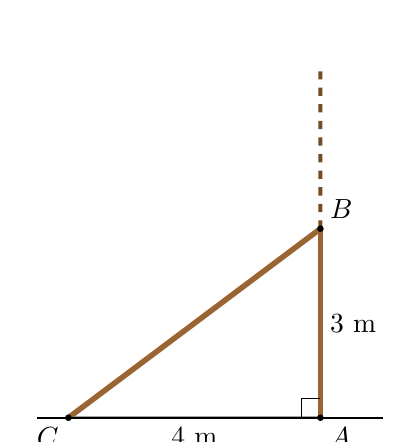
\begin{tikzpicture}[scale=0.8, >=stealth]
  \coordinate (A) at (4,0);
  \coordinate (C) at (0,0);
  \coordinate (B) at (4,3);
  \draw[thick] (C)--(A)--(B)--cycle;
  \draw[dashed, brown!60!black, line width=1.5pt] (B)--(4,5.5);
  \draw[line width=2pt, brown!80!black] (A)--(B);
  \draw[line width=2pt, brown!80!black] (B)--(C);
  \draw[thick] (-0.5,0)--(5,0);
  \fill (A) circle (1.5pt) node[below right] {$A$};
  \fill (B) circle (1.5pt) node[above right] {$B$};
  \fill (C) circle (1.5pt) node[below left] {$C$};
  \draw (3.7,0) |- (4,0.3);
  \node[right] at ($(A)!0.5!(B)$) {$3\text{ m}$};
  \node[below] at ($(A)!0.5!(C)$) {$4\text{ m}$};
\end{tikzpicture}
\end{center}
\begin{enumerate}[label=\textbf{\alph*)}, leftmargin=0.8cm, itemsep=2pt]
\item (0,75 điểm) Tính chiều cao ban đầu của cây cột điện.
\end{enumerate}
\end{ex}
\vspace{0.5mm}

\begin{ex} (0,5 điểm)
Tìm giá trị nhỏ nhất của biểu thức: $P = x^2 + 2y^2 - 2xy - 4y + 2026$.
\begin{enumerate}[label=\textbf{\alph*)}, leftmargin=0.8cm, itemsep=2pt]
\item (0,5 điểm) Tìm giá trị nhỏ nhất của $P$.
\end{enumerate}
\end{ex}
\vspace{0.5mm}


\begin{center}
\rule{4cm}{0.4pt}\\
\textit{--- HẾT ---}
\end{center}
\end{document}
